\documentclass[11pt,a4paper]{article}
\usepackage[utf8]{inputenc}
\usepackage[T1]{fontenc}
\usepackage[spanish,es-tabla]{babel}
\usepackage{graphicx,booktabs,longtable,xcolor,listings,array}
\usepackage[a4paper,margin=2.4cm]{geometry}
\usepackage[colorlinks=true,urlcolor=blue!60!black,linkcolor=black,citecolor=black]{hyperref}
\usepackage{url}
\newcommand{\bdjson}{\lstset{basicstyle=\ttfamily\footnotesize,breaklines=true,frame=single,columns=fullflexible,showstringspaces=false,literate={á}{{\'a}}1 {é}{{\'e}}1 {í}{{\'i}}1 {ó}{{\'o}}1 {ú}{{\'u}}1 {ñ}{{\~n}}1 {Á}{{\'A}}1 {É}{{\'E}}1 {Í}{{\'I}}1 {Ó}{{\'O}}1 {Ú}{{\'U}}1 {→}{{->}}1}}
\bdjson
\newcommand{\cumple}{\textbf{\textcolor{green!45!black}{Cumple}}}
\newcommand{\parcial}{\textbf{\textcolor{orange!80!black}{Parcial}}}
\newcommand{\nocumple}{\textbf{\textcolor{red!70!black}{No cumple}}}
\newcommand{\ev}[1]{\texttt{informe/\allowbreak evidencia/\allowbreak #1}}
\setlength{\parskip}{4pt}
\begin{document}
\begin{titlepage}
\centering
\vspace*{3cm}
{\Large Universidad de Ingeniería y Tecnología (UTEC)\par}
\vspace{1cm}
{\huge\bfseries Informe Final --- CRM de Empleabilidad Nacional\par}
\vspace{1.5cm}
{\Large Curso CS2032 --- Cloud Computing\par}
\vspace{0.5cm}
{\large Grupo 1 \quad|\quad Ciclo 2026-2\par}
\vspace{2cm}
{\large Entrega Semana 15\par}
{\large Fecha de entrega: 22 de noviembre de 2026\par}
\vspace{1cm}
{\normalsize Evidencia recolectada el 17 de noviembre de 2026 (AWS, stage \texttt{dev}, \texttt{us-east-1})\par}
\vspace{1.5cm}
\url{https://github.com/patrickmedina-ds/Proyecto-Final-Cloud-Computing}
\end{titlepage}
\tableofcontents
\newpage
\section{Introducción}
Este informe documenta el proyecto final del curso CS2032 (Cloud Computing, UTEC, ciclo 2026-2): un SaaS multi-tenant tipo CRM de \textbf{empleabilidad nacional}. La plataforma permite que empresas reclutadoras (tenants) administren candidatos, vacantes, postulaciones, entrevistas y reportes mediante cinco microservicios serverless sobre AWS.

\subsection{Alcance y fuentes}
Todas las cifras provienen de la evidencia recolectada el 17 de noviembre de 2026 en \texttt{informe/evidencia/} (archivos 01 a 08, solo lectura sobre AWS salvo las pruebas de API) o del código en \texttt{microservicios/}. Cuando un requisito no se cumple, se declara así de forma explícita (sección~\ref{sec:cumplimiento}).

\begin{tabular}{@{}ll@{}}
\toprule
Dato & Valor \\
\midrule
Tipo de SaaS & CRM de empleabilidad nacional \\
Tenants & \texttt{tenant\_1} (Talento Andino S.A.C.), \texttt{tenant\_2} (Recluta Perú Consultores), \texttt{tenant\_3} \\
Región / runtime & \texttt{us-east-1} / Python 3.11 \\
Framework de despliegue & Serverless Framework v3 \\
Stages desplegados & solo \texttt{dev} \\
Cuenta AWS & AWS Academy (sin Cognito) \\
\bottomrule
\end{tabular}

\subsection{Funcionalidad del CRM}
\begin{tabular}{@{}p{3cm}p{3.2cm}p{7.6cm}@{}}
\toprule
Entidad & Microservicio & Funcionalidad \\
\midrule
Tenant / usuario & usuarios & Alta de usuarios por el administrador, login, refresh y validación de tokens. \\
Candidato & candidatos & CRUD de candidatos y URL prefirmada para subir el CV a S3. \\
Vacante & vacantes & CRUD de vacantes en RDS (un schema por tenant). \\
Postulación & vacantes & CRUD de postulaciones con pipeline de estados (postulado, preseleccionado, entrevista, oferta, contratado, rechazado). \\
Entrevista & entrevistas & CRUD de entrevistas y notificación asíncrona (SNS, SQS, Lambda). \\
Reporte & reportes & Generación y consulta de reportes con conteos del tenant. \\
\bottomrule
\end{tabular}

\section{Arquitectura de la solución}
\subsection{Diagrama}
La figura~\ref{fig:arq} muestra el diagrama de arquitectura (también disponible como \texttt{Diagrama\_\allowbreak Arquitectura\_\allowbreak Solucion.drawio} en la raíz del repositorio). Estado del requisito: \cumple.

\begin{figure}[htbp]
\centering
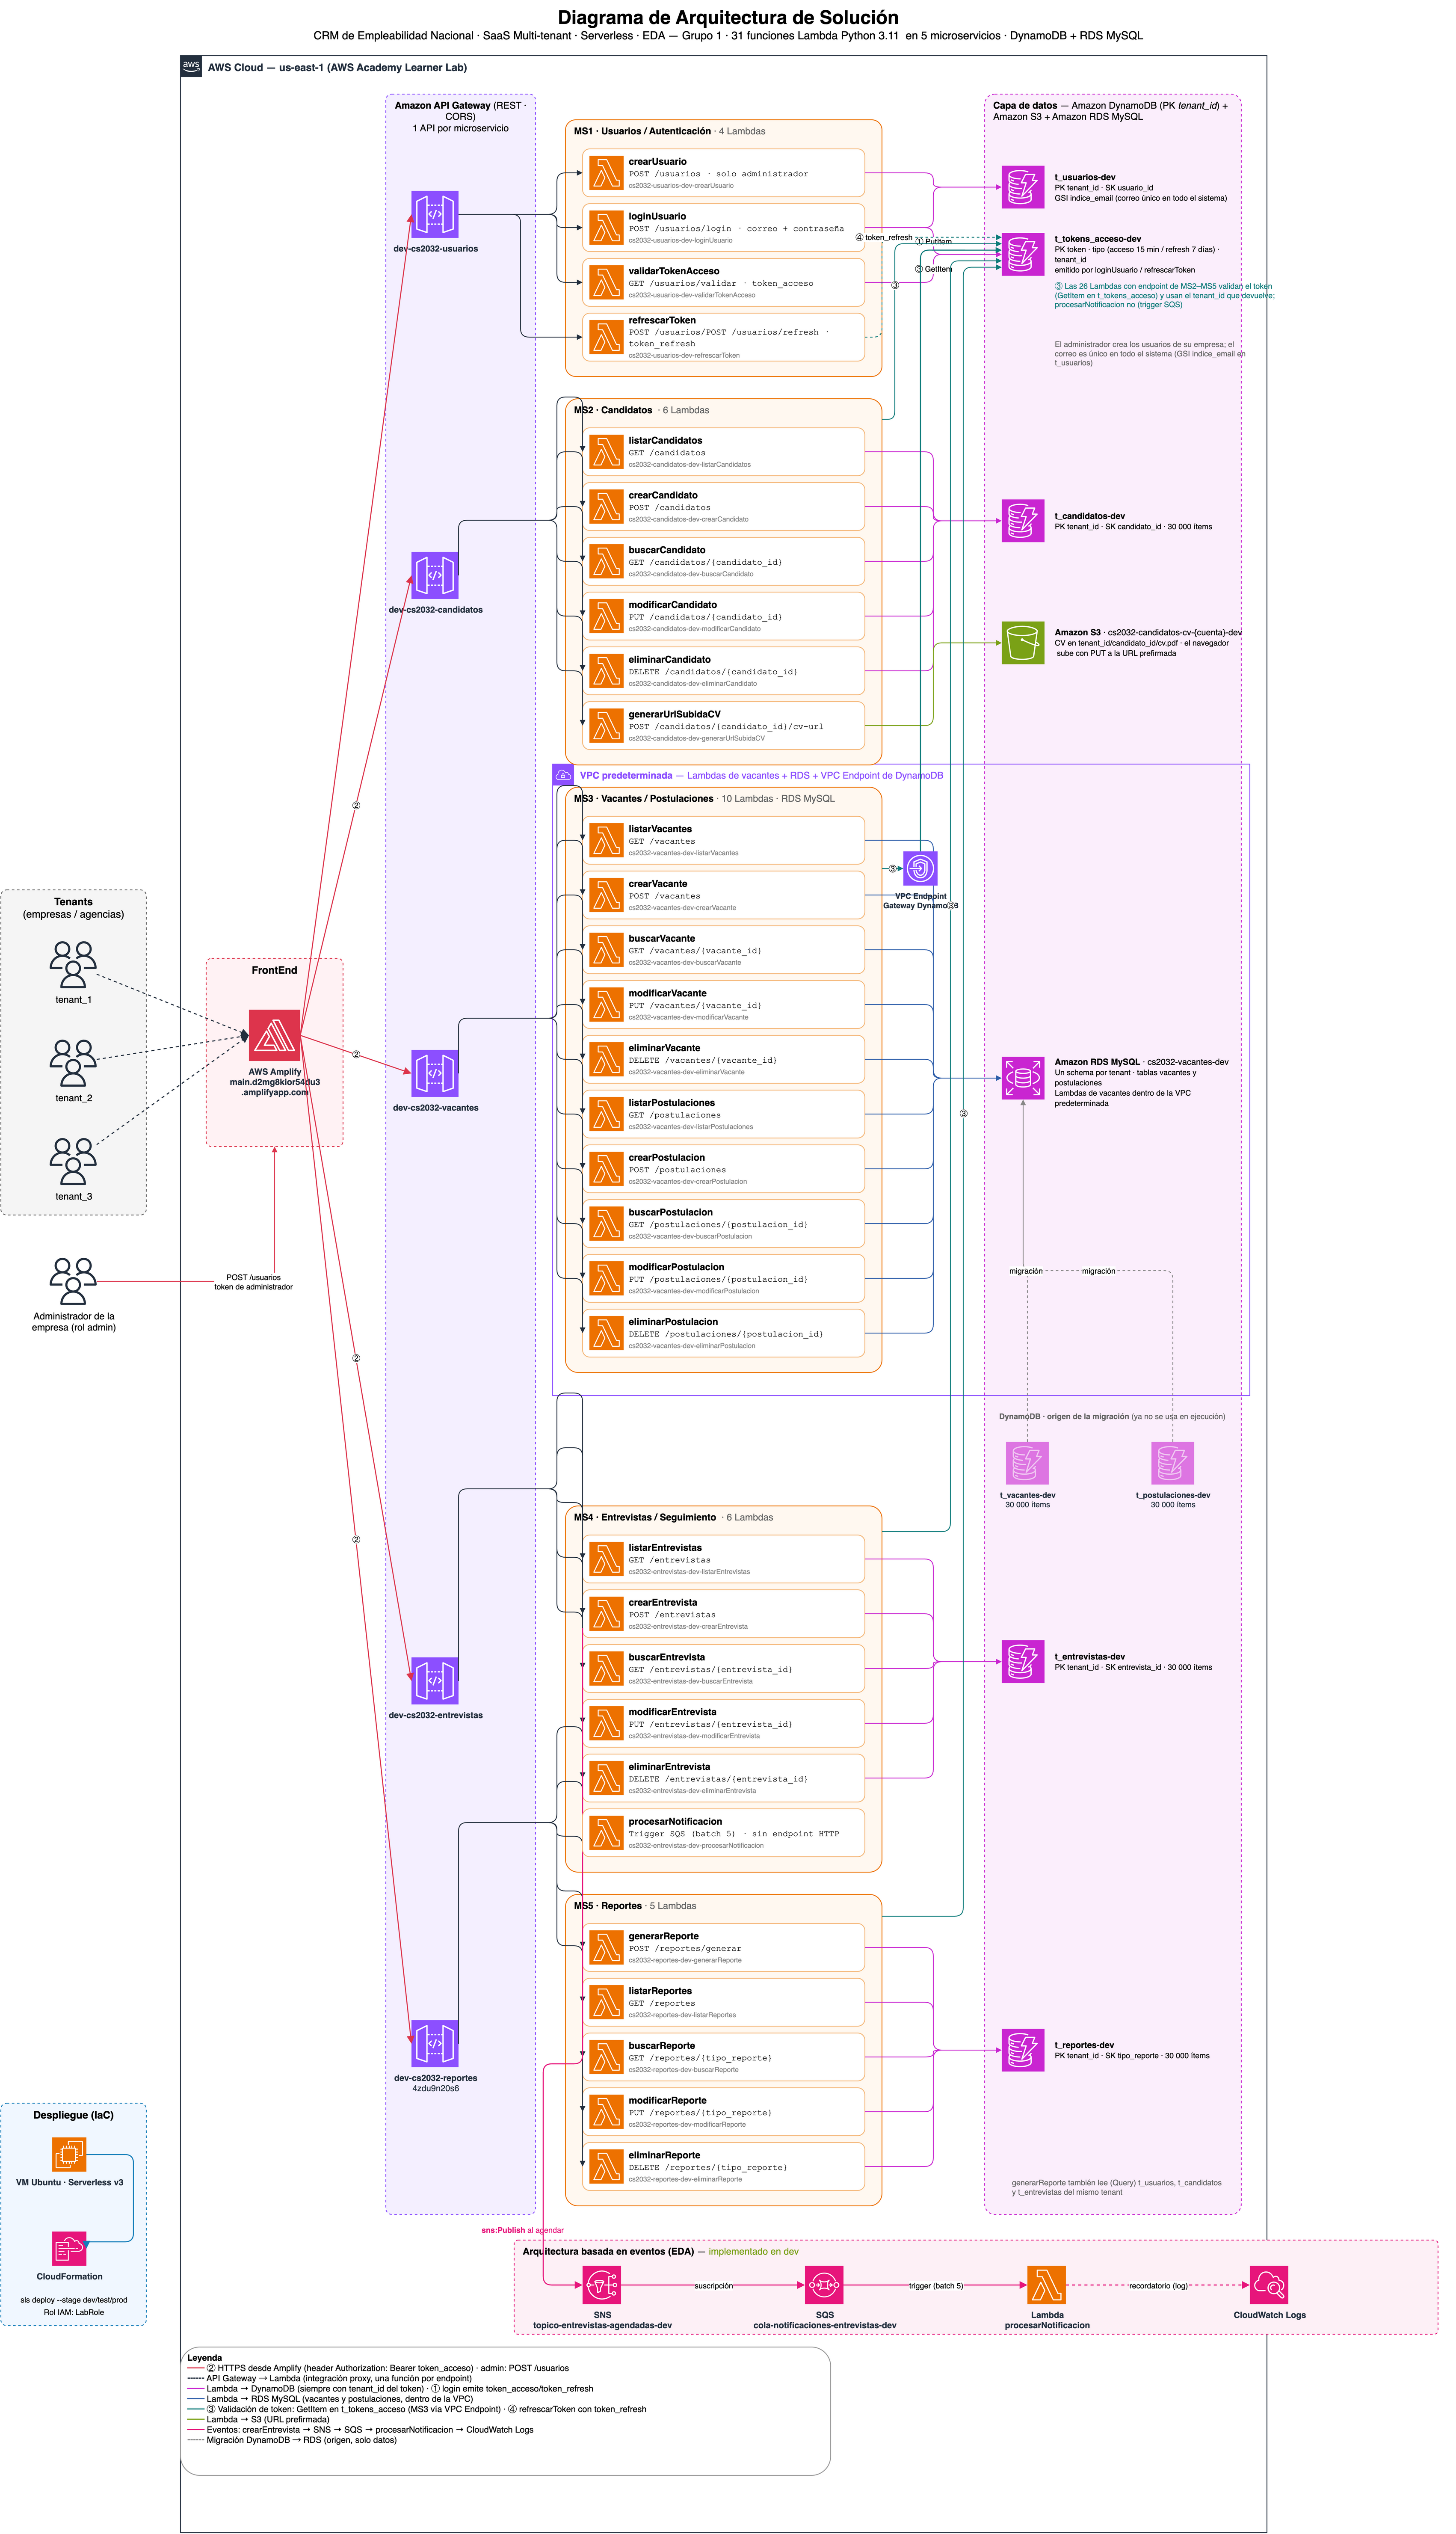
\includegraphics[height=0.82\textheight,width=\textwidth,keepaspectratio]{figuras/Diagrama_Arquitectura_Solucion.png}
\caption{Diagrama de arquitectura de la solución.}\label{fig:arq}
\end{figure}

\subsection{Explicación por capas}
\begin{longtable}{p{3cm}p{11cm}}
\toprule
\textbf{Capa} & \textbf{Componentes} \\
\midrule
\endhead
Presentación & Frontend estático (HTML, CSS, JS) en AWS Amplify, que consume las cinco APIs. \\
API & Cinco APIs REST de API Gateway (\texttt{dev-cs2032-usuarios}, \texttt{-candidatos}, \texttt{-vacantes}, \texttt{-entrevistas}, \texttt{-reportes}). \\
Cómputo & 31 funciones Lambda Python 3.11, una por endpoint, empaquetadas individualmente con un módulo \texttt{common/} compartido. \\
Autenticación & Tablas propias \texttt{t\_usuarios-dev} y \texttt{t\_tokens\_acceso-dev}; cada servicio valida el \texttt{Bearer} con \texttt{get\_item} en la tabla de tokens (no se usa Cognito). \\
Datos & DynamoDB (usuarios, tokens, candidatos, entrevistas, reportes) con \texttt{tenant\_id} como partition key; RDS MySQL 8.0 (vacantes y postulaciones) con un schema por tenant. \\
Almacenamiento & S3: bucket de CVs con URL prefirmada PUT. \\
Mensajería (EDA) & SNS \texttt{topico-entrevistas-agendadas-dev}, SQS \texttt{cola-notificaciones-entrevistas-dev}, Lambda \texttt{procesarNotificacion}. \\
Red & VPC predeterminada \texttt{vpc-0fac6f2d1ab59f1fa}; endpoints de DynamoDB (gateway) y SNS (interface); Lambdas de vacantes, \texttt{crearEntrevista} y \texttt{generarReporte} dentro de la VPC. \\
Despliegue & Serverless Framework v3; un \texttt{serverless.yml} por servicio, un stack CloudFormation por servicio. \\
\bottomrule
\end{longtable}

\subsection{Multi-tenancy}
\begin{itemize}
\item \textbf{DynamoDB:} \texttt{tenant\_id} es partition key de las tablas de negocio; su valor se toma del token validado, nunca del body ni de la URL.
\item \textbf{RDS:} patrón \emph{Single Database, Multiple Schemas}: una instancia \texttt{cs2032-vacantes-dev} (MySQL 8.0.46, db.t3.micro, Single-AZ, no pública, sin cifrado) con un schema por tenant.
\item \textbf{S3:} prefijo \texttt{tenant\_id/candidato\_id/cv.pdf}.
\end{itemize}
Estado: \cumple. La prueba de aislamiento (sección~\ref{sec:pruebas}) confirma que \texttt{tenant\_2} recibe 404 sobre recursos de \texttt{tenant\_1}.

\subsection{Evidencia de red y seguridad}
\ev{05\_vpc\_seguridad.txt}:
\begin{tabular}{@{}lll@{}}
\toprule
Recurso & Identificador & Detalle \\
\midrule
VPC & \texttt{vpc-0fac6f2d1ab59f1fa} & 172.31.0.0/16, available \\
Endpoint DynamoDB & \texttt{vpce-06ffe41b6ff20907a} & Gateway, available \\
Endpoint SNS & \texttt{vpce-0c5e6af041ebd0462} & Interface, available \\
Security group & \texttt{sg-01975563d890002a4} & Entrada solo desde el propio SG (todo y 3306); salida 0.0.0.0/0 \\
\bottomrule
\end{tabular}

% Fragmento para \input: requiere booktabs, longtable y listings (con utf8).
\providecommand{\bdjson}{\lstset{basicstyle=\ttfamily\footnotesize,breaklines=true,frame=single,columns=fullflexible,showstringspaces=false,literate={á}{{\'a}}1 {é}{{\'e}}1 {í}{{\'i}}1 {ó}{{\'o}}1 {ú}{{\'u}}1 {ñ}{{\~n}}1 {Á}{{\'A}}1 {É}{{\'E}}1 {Í}{{\'I}}1 {Ó}{{\'O}}1 {Ú}{{\'U}}1}}
\bdjson
\section{Diseño de bases de datos}
Esta sección describe las bases de datos que usa realmente el código de los cinco microservicios (stage \texttt{dev}, región \texttt{us-\allowbreak{}east-\allowbreak{}1}).

\subsection{Estrategia de multi-tenancy}
\begin{longtable}{p{2.6cm}p{4.4cm}p{7cm}}
\toprule
\textbf{Almacén} & \textbf{Servicios} & \textbf{Aislamiento} \\
\midrule
\endfirsthead
\toprule
\textbf{Almacén} & \textbf{Servicios} & \textbf{Aislamiento} \\
\midrule
\endhead
\bottomrule
\endlastfoot
DynamoDB & usuarios, candidatos, entrevistas, reportes & \texttt{tenant\_\allowbreak{}id} es la partition key de cada tabla de negocio; el valor sale siempre del token validado, nunca del body ni de la URL. \\
RDS MySQL & vacantes y postulaciones (lectura desde entrevistas y reportes) & Patrón Single Database, Multiple Schemas: una instancia con un schema por tenant (\texttt{tenant\_\allowbreak{}1}, \texttt{tenant\_\allowbreak{}2}, \texttt{tenant\_\allowbreak{}3}). \\
S3 & candidatos & Bucket \texttt{cs2032-\allowbreak{}candidatos-\allowbreak{}cv-\allowbreak{}dev-\allowbreak{}\textless{}account-\allowbreak{}id\textgreater{}} con prefijo \texttt{\textless{}tenant\_\allowbreak{}id\textgreater{}/\textless{}candidato\_\allowbreak{}id\textgreater{}/cv.pdf}. \\
\end{longtable}

Todas las tablas DynamoDB usan \texttt{PAY\_\allowbreak{}PER\_\allowbreak{}REQUEST}.

\subsection{Usuarios y autenticación (DynamoDB)}
\subsubsection{Tabla \texttt{t\_usuarios-dev}}
\begin{longtable}{p{3.5cm}p{10.5cm}}
\toprule
\textbf{Elemento} & \textbf{Valor} \\
\midrule
\endfirsthead
\toprule
\textbf{Elemento} & \textbf{Valor} \\
\midrule
\endhead
\bottomrule
\endlastfoot
Partition key & \texttt{tenant\_\allowbreak{}id} (S) \\
Sort key & \texttt{usuario\_\allowbreak{}id} (S, uuid4) \\
GSI \texttt{indice\_\allowbreak{}email} & PK \texttt{email} (S), sin sort key, proyección \texttt{ALL} \\
\end{longtable}

El GSI permite el login sin conocer el tenant: el correo es único en todo el sistema.

\begin{longtable}{p{3.4cm}p{1.2cm}p{1.4cm}p{8cm}}
\caption{Campos de t\_usuarios-dev}\\
\toprule
\textbf{Campo} & \textbf{Tipo} & \textbf{Oblig.} & \textbf{Descripción} \\
\midrule
\endfirsthead
\toprule
\textbf{Campo} & \textbf{Tipo} & \textbf{Oblig.} & \textbf{Descripción} \\
\midrule
\endhead
\bottomrule
\endlastfoot
\texttt{tenant\_\allowbreak{}id} & S & Sí (PK) & Tenant del usuario; sale del token del administrador que lo crea. \\
\texttt{usuario\_\allowbreak{}id} & S & Sí (SK) & uuid4 generado por el servicio. \\
\texttt{nombre} & S & Sí & Texto no vacío. \\
\texttt{email} & S & Sí & Minúsculas; único global (GSI). \\
\texttt{password\_\allowbreak{}hash} & S & Sí & Formato \texttt{pbkdf2\_\allowbreak{}sha256\$310000\$\textless{}salt\_\allowbreak{}hex\textgreater{}\$\textless{}hash\_\allowbreak{}hex\textgreater{}}; los hashes legados sha256 se migran al hacer login. Nunca se devuelve en la API. \\
\texttt{rol} & S & Sí & \texttt{administrador} o \texttt{reclutador} (por defecto \texttt{reclutador}). \\
\texttt{fecha\_\allowbreak{}registro} & S & Sí & ISO 8601 UTC. \\
\end{longtable}

\begin{lstlisting}
{
  "tenant_id": "tenant_1",
  "usuario_id": "3f1c9a52-7b0e-4d6a-9a8e-0c5d2b7f4e11",
  "nombre": "Lucía Ramos",
  "email": "lucia.ramos@empresa1.example",
  "password_hash": "pbkdf2_sha256$310000$9f2a...c1$5be0...7d",
  "rol": "administrador",
  "fecha_registro": "2026-10-02T14:31:08.512340+00:00"
}
\end{lstlisting}

\subsubsection{Tabla \texttt{t\_tokens\_acceso-dev}}
\begin{longtable}{p{3.5cm}p{10.5cm}}
\toprule
\textbf{Elemento} & \textbf{Valor} \\
\midrule
\endfirsthead
\toprule
\textbf{Elemento} & \textbf{Valor} \\
\midrule
\endhead
\bottomrule
\endlastfoot
Partition key & \texttt{token} (S, uuid4) \\
Sort key & No tiene \\
GSI & No tiene \\
TTL & Atributo \texttt{ttl} habilitado \\
\end{longtable}

Usa \texttt{token} como partition key porque cada petición llega solo con el token; cada item guarda el \texttt{tenant\_\allowbreak{}id}. Es la tabla que leen todos los microservicios. Se emiten tokens \texttt{acceso} (15 minutos) y \texttt{refresh} (7 días).

\begin{longtable}{p{3.4cm}p{1.2cm}p{1.4cm}p{8cm}}
\caption{Campos de t\_tokens\_acceso-dev}\\
\toprule
\textbf{Campo} & \textbf{Tipo} & \textbf{Oblig.} & \textbf{Descripción} \\
\midrule
\endfirsthead
\toprule
\textbf{Campo} & \textbf{Tipo} & \textbf{Oblig.} & \textbf{Descripción} \\
\midrule
\endhead
\bottomrule
\endlastfoot
\texttt{token} & S & Sí (PK) & uuid4. \\
\texttt{tipo} & S & Sí & \texttt{acceso} o \texttt{refresh}; un refresh no sirve en endpoints protegidos. \\
\texttt{tenant\_\allowbreak{}id} & S & Sí & Tenant del usuario. \\
\texttt{usuario\_\allowbreak{}id} & S & Sí & Usuario dueño del token. \\
\texttt{expira} & N & Sí & Epoch en segundos; se compara con la hora actual. \\
\texttt{ttl} & N & Sí & Igual a \texttt{expira}; DynamoDB borra el item al vencer. \\
\texttt{fecha\_\allowbreak{}expiracion} & S & Sí & ISO 8601, por compatibilidad. \\
\end{longtable}

\begin{lstlisting}
{
  "token": "b7d3e0a4-52c1-4f7e-8d90-1a6c3e9f2b48",
  "tipo": "acceso",
  "tenant_id": "tenant_1",
  "usuario_id": "3f1c9a52-7b0e-4d6a-9a8e-0c5d2b7f4e11",
  "expira": 1795012345,
  "ttl": 1795012345,
  "fecha_expiracion": "2026-11-17T15:12:25+00:00"
}
\end{lstlisting}

\subsection{Candidatos (DynamoDB y S3)}
\subsubsection{Tabla \texttt{t\_candidatos-dev}}
\begin{longtable}{p{3.5cm}p{10.5cm}}
\toprule
\textbf{Elemento} & \textbf{Valor} \\
\midrule
\endfirsthead
\toprule
\textbf{Elemento} & \textbf{Valor} \\
\midrule
\endhead
\bottomrule
\endlastfoot
Partition key & \texttt{tenant\_\allowbreak{}id} (S) \\
Sort key & \texttt{candidato\_\allowbreak{}id} (S, uuid4) \\
GSI & Ninguno \\
\end{longtable}

\begin{longtable}{p{3.4cm}p{1.2cm}p{1.4cm}p{8cm}}
\caption{Campos de t\_candidatos-dev}\\
\toprule
\textbf{Campo} & \textbf{Tipo} & \textbf{Oblig.} & \textbf{Descripción} \\
\midrule
\endfirsthead
\toprule
\textbf{Campo} & \textbf{Tipo} & \textbf{Oblig.} & \textbf{Descripción} \\
\midrule
\endhead
\bottomrule
\endlastfoot
\texttt{tenant\_\allowbreak{}id} & S & Sí (PK) & Del token. \\
\texttt{candidato\_\allowbreak{}id} & S & Sí (SK) & uuid4. \\
\texttt{nombre} & S & Sí & Texto no vacío. \\
\texttt{email} & S & Sí & Debe contener \texttt{@}. \\
\texttt{telefono} & S & Sí & Texto no vacío. \\
\texttt{profesion} & S & Sí & Texto no vacío. \\
\texttt{estado} & S & Sí & \texttt{activo} o \texttt{inactivo}; el alta lo fija en \texttt{activo}. \\
\texttt{cv\_\allowbreak{}url} & S & Sí & Cadena vacía al crear; luego guarda la key S3 \texttt{\textless{}tenant\_\allowbreak{}id\textgreater{}/\textless{}candidato\_\allowbreak{}id\textgreater{}/cv.pdf} (no una URL). \\
\texttt{fecha\_\allowbreak{}registro} & S & Sí & ISO 8601 UTC. \\
\texttt{fecha\_\allowbreak{}actualizacion} & S & Sí & ISO 8601 UTC. \\
\end{longtable}

\begin{lstlisting}
{
  "tenant_id": "tenant_1",
  "candidato_id": "8a41d7c0-3e5b-4c29-b1f6-72d09e4a5c33",
  "nombre": "Carlos Pérez Soto",
  "email": "carlos.perez@correo.example",
  "telefono": "987654321",
  "profesion": "Ingeniero de software",
  "estado": "activo",
  "cv_url": "tenant_1/8a41d7c0-3e5b-4c29-b1f6-72d09e4a5c33/cv.pdf",
  "fecha_registro": "2026-09-14T10:05:41.220113+00:00",
  "fecha_actualizacion": "2026-09-20T16:48:02.774901+00:00"
}
\end{lstlisting}

El PDF se guarda en el bucket S3 \texttt{cs2032-\allowbreak{}candidatos-\allowbreak{}cv-\allowbreak{}dev-\allowbreak{}\textless{}account-\allowbreak{}id\textgreater{}} mediante una URL prefirmada de 300 segundos.

\subsection{Vacantes y postulaciones (RDS MySQL)}
\subsubsection{Patrón Single Database, Multiple Schemas}
Existe una única instancia RDS MySQL (\texttt{\textless{}host-\allowbreak{}rds\textgreater{}}, puerto 3306) con un schema por tenant (\texttt{tenant\_\allowbreak{}1}, \texttt{tenant\_\allowbreak{}2}, \texttt{tenant\_\allowbreak{}3}); cada schema contiene las mismas tablas \texttt{vacantes} y \texttt{postulaciones}. El aislamiento funciona así:
\begin{itemize}
\item El \texttt{tenant\_\allowbreak{}id} del token decide el schema: \texttt{common/rds.py} valida el patrón \texttt{\^{}tenant\_\allowbreak{}[a-\allowbreak{}z0-\allowbreak{}9\_\allowbreak{}]+\$} y lo pasa solo como parámetro \texttt{database} de la conexión, nunca dentro del SQL.
\item Las consultas no filtran por tenant porque ya ejecutan en el schema correcto; todas son parametrizadas y las columnas editables van en listas blancas.
\item La clave foránea \texttt{postulaciones.vacante\_\allowbreak{}id} hacia \texttt{vacantes.vacante\_\allowbreak{}id} es dentro del mismo schema; eliminar una vacante con postulaciones devuelve 409 (sin borrado en cascada).
\item \texttt{postulaciones.candidato\_\allowbreak{}id} no es clave foránea: el candidato vive en DynamoDB y se valida por código.
\end{itemize}

\subsubsection{Relación entre entidades}
Relación 1 a N: una \texttt{vacantes} recibe cero o más \texttt{postulaciones} (\texttt{postulaciones.vacante\_\allowbreak{}id} FK hacia \texttt{vacantes.vacante\_\allowbreak{}id}).

\subsubsection{Entidad \texttt{vacantes}}
\begin{longtable}{p{3cm}p{2.7cm}p{3.6cm}p{4.7cm}}
\caption{Entidad vacantes}\\
\toprule
\textbf{Campo} & \textbf{Tipo} & \textbf{Restricción} & \textbf{Descripción} \\
\midrule
\endfirsthead
\toprule
\textbf{Campo} & \textbf{Tipo} & \textbf{Restricción} & \textbf{Descripción} \\
\midrule
\endhead
\bottomrule
\endlastfoot
\texttt{vacante\_\allowbreak{}id} & CHAR(36) & PRIMARY KEY & uuid4. \\
\texttt{titulo} & VARCHAR(150) & NOT NULL & Obligatorio al crear. \\
\texttt{descripcion} & TEXT & NULL & Obligatoria al crear (validación del handler). \\
\texttt{area} & VARCHAR(100) & NULL & Opcional. \\
\texttt{ubicacion} & VARCHAR(100) & NULL & Opcional. \\
\texttt{modalidad} & VARCHAR(20) & NOT NULL, DEFAULT 'presencial' & \texttt{presencial}, \texttt{remoto} o \texttt{hibrido}. \\
\texttt{salario} & DECIMAL(12,2) & NULL & Número mayor o igual a 0. \\
\texttt{candidato\_\allowbreak{}id} & CHAR(36) & NULL & Heredada del documento original; el código no la escribe. \\
\texttt{estado} & VARCHAR(30) & NOT NULL, DEFAULT 'abierta' & \texttt{abierta} o \texttt{cerrada}; se crea siempre \texttt{abierta}. \\
\texttt{fecha\_\allowbreak{}publicacion} & DATETIME & NULL & UTC; se fija al crear. \\
\texttt{fecha\_\allowbreak{}actualizacion} & DATETIME & NULL & UTC; cambia en cada modificación. \\
\end{longtable}

\subsubsection{Entidad \texttt{postulaciones}}
\begin{longtable}{p{3cm}p{2.7cm}p{3.6cm}p{4.7cm}}
\caption{Entidad postulaciones}\\
\toprule
\textbf{Campo} & \textbf{Tipo} & \textbf{Restricción} & \textbf{Descripción} \\
\midrule
\endfirsthead
\toprule
\textbf{Campo} & \textbf{Tipo} & \textbf{Restricción} & \textbf{Descripción} \\
\midrule
\endhead
\bottomrule
\endlastfoot
\texttt{postulacion\_\allowbreak{}id} & CHAR(36) & PRIMARY KEY & uuid4. \\
\texttt{vacante\_\allowbreak{}id} & CHAR(36) & NOT NULL, FK a vacantes, INDEX indice\_vacante & La vacante debe existir y estar \texttt{abierta}. \\
\texttt{candidato\_\allowbreak{}id} & CHAR(36) & NOT NULL & Se valida contra DynamoDB \texttt{t\_\allowbreak{}candidatos-\allowbreak{}dev}. \\
\texttt{titulo\_\allowbreak{}vacante} & VARCHAR(150) & NULL & Copia del título al postular. \\
\texttt{estado} & VARCHAR(30) & NOT NULL, DEFAULT 'postulado', INDEX indice\_estado & \texttt{postulado}, \texttt{preseleccionado}, \texttt{entrevista}, \texttt{oferta}, \texttt{contratado}, \texttt{rechazado}. \\
\texttt{notas} & TEXT & NULL & Texto libre; solo \texttt{estado} y \texttt{notas} son modificables. \\
\texttt{fecha\_\allowbreak{}postulacion} & DATETIME & NULL & UTC. \\
\texttt{fecha\_\allowbreak{}actualizacion} & DATETIME & NULL & UTC. \\
\end{longtable}

\subsubsection{DDL resumido}
\begin{lstlisting}
CREATE SCHEMA IF NOT EXISTS tenant_1;  -- idem tenant_2, tenant_3

CREATE TABLE tenant_1.vacantes (
  vacante_id CHAR(36) PRIMARY KEY,
  titulo VARCHAR(150) NOT NULL,
  descripcion TEXT, area VARCHAR(100), ubicacion VARCHAR(100),
  modalidad VARCHAR(20) NOT NULL DEFAULT 'presencial',
  salario DECIMAL(12,2), candidato_id CHAR(36),
  estado VARCHAR(30) NOT NULL DEFAULT 'abierta',
  fecha_publicacion DATETIME, fecha_actualizacion DATETIME
);
CREATE TABLE tenant_1.postulaciones (
  postulacion_id CHAR(36) PRIMARY KEY,
  vacante_id CHAR(36) NOT NULL,
  candidato_id CHAR(36) NOT NULL,
  titulo_vacante VARCHAR(150),
  estado VARCHAR(30) NOT NULL DEFAULT 'postulado',
  notas TEXT,
  fecha_postulacion DATETIME, fecha_actualizacion DATETIME,
  INDEX indice_estado (estado),
  INDEX indice_vacante (vacante_id),
  FOREIGN KEY (vacante_id) REFERENCES tenant_1.vacantes (vacante_id)
);
\end{lstlisting}

\subsubsection{Ejemplos}
\begin{lstlisting}
{
  "tenant_id": "tenant_1",
  "vacante_id": "c2e84b90-1d7a-4f35-a6c8-9e0b3d5f7a12",
  "titulo": "Analista de datos",
  "descripcion": "Responsable de tableros y reportes de selección.",
  "area": "datos", "ubicacion": "Lima", "modalidad": "hibrido",
  "salario": 4500.0, "estado": "abierta",
  "fecha_publicacion": "2026-10-05T09:00:00+00:00",
  "fecha_actualizacion": "2026-10-05T09:00:00+00:00"
}
\end{lstlisting}

\begin{lstlisting}
{
  "tenant_id": "tenant_1",
  "postulacion_id": "5d90f1b7-6a3c-4e82-8f14-b27c0a9d3e66",
  "vacante_id": "c2e84b90-1d7a-4f35-a6c8-9e0b3d5f7a12",
  "candidato_id": "8a41d7c0-3e5b-4c29-b1f6-72d09e4a5c33",
  "titulo_vacante": "Analista de datos",
  "estado": "preseleccionado",
  "notas": "Cumple el perfil técnico.",
  "fecha_postulacion": "2026-10-06T11:20:00+00:00",
  "fecha_actualizacion": "2026-10-08T15:45:30+00:00"
}
\end{lstlisting}

La API añade \texttt{tenant\_\allowbreak{}id} (tomado del token) y omite los valores NULL.

\subsubsection{Tablas DynamoDB heredadas}
El \texttt{serverless.yml} de vacantes aún declara \texttt{t\_\allowbreak{}vacantes-\allowbreak{}dev} (PK \texttt{tenant\_\allowbreak{}id}, SK \texttt{vacante\_\allowbreak{}id}) y \texttt{t\_\allowbreak{}postulaciones-\allowbreak{}dev} (PK \texttt{tenant\_\allowbreak{}id}, SK \texttt{postulacion\_\allowbreak{}id}; GSI \texttt{indice\_\allowbreak{}estado} = \texttt{tenant\_\allowbreak{}id} + \texttt{estado} e \texttt{indice\_\allowbreak{}vacante} = \texttt{tenant\_\allowbreak{}id} + \texttt{vacante\_\allowbreak{}id}, ambos con proyección \texttt{ALL}). Los handlers actuales no las leen ni escriben: fueron la fuente de la migración a RDS y los scripts de carga de entrevistas todavía las consultan. Los índices de RDS reemplazan a esos GSI.

\subsection{Entrevistas (DynamoDB)}
\subsubsection{Tabla \texttt{t\_entrevistas-dev}}
\begin{longtable}{p{3.5cm}p{10.5cm}}
\toprule
\textbf{Elemento} & \textbf{Valor} \\
\midrule
\endfirsthead
\toprule
\textbf{Elemento} & \textbf{Valor} \\
\midrule
\endhead
\bottomrule
\endlastfoot
Partition key & \texttt{tenant\_\allowbreak{}id} (S) \\
Sort key & \texttt{entrevista\_\allowbreak{}id} (S, uuid4) \\
GSI & Ninguno (los filtros por \texttt{estado}, \texttt{candidato\_\allowbreak{}id} y \texttt{vacante\_\allowbreak{}id} usan FilterExpression sobre un Query por tenant) \\
\end{longtable}

\begin{longtable}{p{3.4cm}p{1.2cm}p{1.4cm}p{8cm}}
\caption{Campos de t\_entrevistas-dev}\\
\toprule
\textbf{Campo} & \textbf{Tipo} & \textbf{Oblig.} & \textbf{Descripción} \\
\midrule
\endfirsthead
\toprule
\textbf{Campo} & \textbf{Tipo} & \textbf{Oblig.} & \textbf{Descripción} \\
\midrule
\endhead
\bottomrule
\endlastfoot
\texttt{tenant\_\allowbreak{}id} & S & Sí (PK) & Del token. \\
\texttt{entrevista\_\allowbreak{}id} & S & Sí (SK) & uuid4. \\
\texttt{candidato\_\allowbreak{}id} & S & Sí & Se valida en DynamoDB \texttt{t\_\allowbreak{}candidatos-\allowbreak{}dev}. \\
\texttt{vacante\_\allowbreak{}id} & S & Sí & Se valida en RDS (\texttt{SELECT 1 FROM vacantes} en el schema del tenant). \\
\texttt{postulacion\_\allowbreak{}id} & S & No & Cadena vacía si no se envía. \\
\texttt{entrevistador} & S & Sí & Texto no vacío. \\
\texttt{fecha\_\allowbreak{}hora} & S & Sí & ISO 8601 con zona. \\
\texttt{modalidad} & S & Sí & \texttt{presencial} o \texttt{virtual}. \\
\texttt{estado} & S & Sí & \texttt{agendada} (al crear), \texttt{realizada} o \texttt{cancelada}. \\
\texttt{notas} & S & Sí & Cadena vacía al crear. \\
\texttt{fecha\_\allowbreak{}creacion} & S & Sí & ISO 8601 UTC. \\
\texttt{fecha\_\allowbreak{}actualizacion} & S & Sí & ISO 8601 UTC. \\
\end{longtable}

\begin{lstlisting}
{
  "tenant_id": "tenant_1",
  "entrevista_id": "e19a6c3d-0b84-4a7f-93d2-5c8f1e0b7a29",
  "candidato_id": "8a41d7c0-3e5b-4c29-b1f6-72d09e4a5c33",
  "vacante_id": "c2e84b90-1d7a-4f35-a6c8-9e0b3d5f7a12",
  "postulacion_id": "5d90f1b7-6a3c-4e82-8f14-b27c0a9d3e66",
  "entrevistador": "Marta Quispe",
  "fecha_hora": "2026-11-20T15:00:00-05:00",
  "modalidad": "virtual",
  "estado": "agendada",
  "notas": "",
  "fecha_creacion": "2026-11-12T13:02:10.318822+00:00",
  "fecha_actualizacion": "2026-11-12T13:02:10.318822+00:00"
}
\end{lstlisting}

Recursos de mensajería asociados: tópico SNS \texttt{topico-\allowbreak{}entrevistas-\allowbreak{}agendadas-\allowbreak{}dev} y cola SQS \texttt{cola-\allowbreak{}notificaciones-\allowbreak{}entrevistas-\allowbreak{}dev}; el evento \texttt{entrevista\_\allowbreak{}agendada} lleva \texttt{tenant\_\allowbreak{}id}, \texttt{entrevista\_\allowbreak{}id}, \texttt{candidato\_\allowbreak{}id}, \texttt{vacante\_\allowbreak{}id}, \texttt{fecha\_\allowbreak{}hora}, \texttt{modalidad} y \texttt{entrevistador}.

\subsection{Reportes (DynamoDB)}
\subsubsection{Tabla \texttt{t\_reportes-dev}}
\begin{longtable}{p{3.5cm}p{10.5cm}}
\toprule
\textbf{Elemento} & \textbf{Valor} \\
\midrule
\endfirsthead
\toprule
\textbf{Elemento} & \textbf{Valor} \\
\midrule
\endhead
\bottomrule
\endlastfoot
Partition key & \texttt{tenant\_\allowbreak{}id} (S) \\
Sort key & \texttt{tipo\_\allowbreak{}reporte} (S) \\
GSI & Ninguno \\
\end{longtable}

\texttt{POST /reportes/generar} guarda un item con \texttt{tipo\_\allowbreak{}reporte} = \texttt{resumen\_\allowbreak{}general} (uno por tenant, se sobrescribe). El script \texttt{scripts/cargar\_\allowbreak{}datos.py} siembra además reportes diarios con \texttt{tipo\_\allowbreak{}reporte} = \texttt{diario\_\allowbreak{}\textless{}fecha\textgreater{}\_\allowbreak{}\textless{}area\textgreater{}}.

\begin{longtable}{p{4cm}p{1.2cm}p{1.4cm}p{7.4cm}}
\caption{Campos del item resumen\_general}\\
\toprule
\textbf{Campo} & \textbf{Tipo} & \textbf{Oblig.} & \textbf{Descripción} \\
\midrule
\endfirsthead
\toprule
\textbf{Campo} & \textbf{Tipo} & \textbf{Oblig.} & \textbf{Descripción} \\
\midrule
\endhead
\bottomrule
\endlastfoot
\texttt{tenant\_\allowbreak{}id} & S & Sí (PK) & Del token. \\
\texttt{tipo\_\allowbreak{}reporte} & S & Sí (SK) & \texttt{resumen\_\allowbreak{}general}. \\
\texttt{total\_\allowbreak{}usuarios} & N & Sí & Conteo en \texttt{t\_\allowbreak{}usuarios-\allowbreak{}dev}. \\
\texttt{total\_\allowbreak{}candidatos} & N & Sí & Conteo en \texttt{t\_\allowbreak{}candidatos-\allowbreak{}dev}. \\
\texttt{total\_\allowbreak{}vacantes} & N & Sí & Suma de \texttt{vacantes\_\allowbreak{}por\_\allowbreak{}estado} (RDS). \\
\texttt{vacantes\_\allowbreak{}por\_\allowbreak{}estado} & M & Sí & \texttt{\{estado: conteo\}} desde RDS. \\
\texttt{total\_\allowbreak{}postulaciones} & N & Sí & Suma de \texttt{postulaciones\_\allowbreak{}por\_\allowbreak{}estado} (RDS). \\
\texttt{postulaciones\_\allowbreak{}por\_\allowbreak{}estado} & M & Sí & \texttt{\{estado: conteo\}} desde RDS. \\
\texttt{total\_\allowbreak{}entrevistas} & N & Sí & Suma de \texttt{entrevistas\_\allowbreak{}por\_\allowbreak{}estado}. \\
\texttt{entrevistas\_\allowbreak{}por\_\allowbreak{}estado} & M & Sí & \texttt{\{estado: conteo\}} desde \texttt{t\_\allowbreak{}entrevistas-\allowbreak{}dev}. \\
\texttt{total\_\allowbreak{}contratados} & N & Sí & Postulaciones en estado \texttt{contratado}. \\
\texttt{tasa\_\allowbreak{}contratacion} & N & Sí & Contratados por 100 entre total de postulaciones, 2 decimales (0 si no hay). \\
\texttt{observaciones} & S & Sí & Vacía al generar; es lo único que modifica \texttt{PUT /reportes/\{tipo\_\allowbreak{}reporte\}}. \\
\texttt{fecha\_\allowbreak{}actualizacion} & S & Sí & ISO 8601 UTC. \\
\end{longtable}

\begin{lstlisting}
{
  "tenant_id": "tenant_1",
  "tipo_reporte": "resumen_general",
  "total_usuarios": 4,
  "total_candidatos": 10000,
  "total_vacantes": 10000,
  "vacantes_por_estado": { "abierta": 8200, "cerrada": 1800 },
  "total_postulaciones": 10000,
  "postulaciones_por_estado": { "postulado": 4100, "preseleccionado": 2300,
    "entrevista": 1500, "oferta": 800, "contratado": 700, "rechazado": 600 },
  "total_entrevistas": 10000,
  "entrevistas_por_estado": { "agendada": 1500, "realizada": 7300, "cancelada": 1200 },
  "total_contratados": 700,
  "tasa_contratacion": 7.0,
  "observaciones": "",
  "fecha_actualizacion": "2026-11-17T12:00:00+00:00"
}
\end{lstlisting}

Item diario sembrado por el script (misma clave, otros atributos):

\begin{lstlisting}
{
  "tenant_id": "tenant_1",
  "tipo_reporte": "diario_2026-11-10_datos",
  "fecha": "2026-11-10", "area": "datos",
  "nuevos_candidatos": 31, "nuevas_vacantes": 4,
  "total_postulaciones": 22, "total_entrevistas": 9,
  "total_contratados": 2, "tasa_contratacion": 9.09,
  "observaciones": "",
  "fecha_actualizacion": "2026-11-11T02:00:00+00:00"
}
\end{lstlisting}

\subsection{Relación entre microservicios}
\begin{longtable}{p{2.8cm}p{4.6cm}p{6.6cm}}
\toprule
\textbf{Servicio} & \textbf{Escribe} & \textbf{Lee de otros} \\
\midrule
\endfirsthead
\toprule
\textbf{Servicio} & \textbf{Escribe} & \textbf{Lee de otros} \\
\midrule
\endhead
\bottomrule
\endlastfoot
Usuarios & \texttt{t\_\allowbreak{}usuarios-\allowbreak{}dev}, \texttt{t\_\allowbreak{}tokens\_\allowbreak{}acceso-\allowbreak{}dev} & Ninguno. \\
Candidatos & \texttt{t\_\allowbreak{}candidatos-\allowbreak{}dev}, bucket S3 de CVs & \texttt{t\_\allowbreak{}tokens\_\allowbreak{}acceso-\allowbreak{}dev} (validación de token). \\
Vacantes / postulaciones & RDS: \texttt{vacantes}, \texttt{postulaciones} (schema del tenant) & \texttt{t\_\allowbreak{}candidatos-\allowbreak{}dev} (GetItem para validar \texttt{candidato\_\allowbreak{}id}); \texttt{t\_\allowbreak{}tokens\_\allowbreak{}acceso-\allowbreak{}dev}. \\
Entrevistas & \texttt{t\_\allowbreak{}entrevistas-\allowbreak{}dev}; publica en SNS & \texttt{t\_\allowbreak{}candidatos-\allowbreak{}dev} (GetItem); RDS \texttt{vacantes} (SELECT 1); \texttt{t\_\allowbreak{}tokens\_\allowbreak{}acceso-\allowbreak{}dev}. \\
Reportes & \texttt{t\_\allowbreak{}reportes-\allowbreak{}dev} & RDS \texttt{vacantes} y \texttt{postulaciones} (COUNT por estado); \texttt{t\_\allowbreak{}usuarios-\allowbreak{}dev}, \texttt{t\_\allowbreak{}candidatos-\allowbreak{}dev} y \texttt{t\_\allowbreak{}entrevistas-\allowbreak{}dev} (Query por \texttt{tenant\_\allowbreak{}id}); \texttt{t\_\allowbreak{}tokens\_\allowbreak{}acceso-\allowbreak{}dev}. \\
\end{longtable}

Las referencias entre servicios (\texttt{candidato\_\allowbreak{}id}, \texttt{vacante\_\allowbreak{}id}, \texttt{postulacion\_\allowbreak{}id}) son lógicas: se validan por código, no con claves foráneas, salvo \texttt{postulaciones.vacante\_\allowbreak{}id} hacia \texttt{vacantes.vacante\_\allowbreak{}id} dentro de RDS.

\section{Microservicios serverless}
Requisito: API Gateway + Lambda Python 3.11, mínimo cinco microservicios protegidos. Estado: \cumple. Evidencia: \ev{01\_lambdas.txt}, \ev{02\_api\_gateway.txt}, \ev{06\_cloudformation.txt}.

\subsection{Resumen}
\begin{longtable}{p{2.3cm}p{2.7cm}p{1.6cm}p{2.2cm}p{4.2cm}}
\toprule
\textbf{Servicio} & \textbf{API Gateway} & \textbf{Lambdas} & \textbf{Stack CFN} & \textbf{Datos} \\
\midrule
\endhead
usuarios & \texttt{dev-cs2032-usuarios} (\texttt{jas1g5t9tl}) & 4 & \texttt{cs2032-usuarios-dev} & DynamoDB \\
candidatos & \texttt{dev-cs2032-candidatos} (\texttt{celozfy9cj}) & 6 & \texttt{cs2032-candidatos-dev} & DynamoDB, S3 \\
vacantes & \texttt{dev-cs2032-vacantes} (\texttt{lx1fmyf70f}) & 10 & \texttt{cs2032-vacantes-dev} & RDS MySQL \\
entrevistas & \texttt{dev-cs2032-entrevistas} (\texttt{ik4kelr8a2}) & 6 & \texttt{cs2032-entrevistas-dev} & DynamoDB, SNS, SQS \\
reportes & \texttt{dev-cs2032-reportes} (\texttt{4zdu9n20s6}) & 5 & \texttt{cs2032-reportes-dev} & DynamoDB \\
\midrule
\textbf{Total} & 5 APIs & \textbf{31} & 5 stacks & \\
\bottomrule
\end{longtable}
Los cinco stacks están en \texttt{UPDATE\_COMPLETE} (evidencia 06). Las 31 funciones usan \texttt{python3.11}.

\subsection{Endpoints y Lambdas por servicio}
Todos los endpoints, salvo \texttt{POST /usuarios/login} y \texttt{POST /usuarios/refresh}, exigen \texttt{Authorization: Bearer <token\_acceso>}. Cada recurso tiene además método \texttt{OPTIONS} (CORS).

\begin{longtable}{p{1.9cm}p{5.1cm}p{6.8cm}}
\toprule
\textbf{Servicio} & \textbf{Endpoint} & \textbf{Lambda} \\
\midrule
\endhead
usuarios & \texttt{POST /usuarios} & \texttt{crearUsuario} (solo administrador) \\
 & \texttt{POST /usuarios/login} & \texttt{loginUsuario} \\
 & \texttt{POST /usuarios/refresh} & \texttt{refrescarToken} \\
 & \texttt{GET /usuarios/validar} & \texttt{validarTokenAcceso} \\
\midrule
candidatos & \texttt{GET, POST /candidatos} & \texttt{listarCandidatos}, \texttt{crearCandidato} \\
 & \texttt{GET, PUT, DELETE /candidatos/\{candidato\_id\}} & \texttt{buscarCandidato}, \texttt{modificarCandidato}, \texttt{eliminarCandidato} \\
 & \texttt{POST /candidatos/\{candidato\_id\}/cv-url} & \texttt{generarUrlSubidaCV} \\
\midrule
vacantes & \texttt{GET, POST /vacantes} & \texttt{listarVacantes}, \texttt{crearVacante} \\
 & \texttt{GET, PUT, DELETE /vacantes/\{vacante\_id\}} & \texttt{buscarVacante}, \texttt{modificarVacante}, \texttt{eliminarVacante} \\
 & \texttt{GET, POST /postulaciones} & \texttt{listarPostulaciones}, \texttt{crearPostulacion} \\
 & \texttt{GET, PUT, DELETE /postulaciones/\{postulacion\_id\}} & \texttt{buscarPostulacion}, \texttt{modificarPostulacion}, \texttt{eliminarPostulacion} \\
\midrule
entrevistas & \texttt{GET, POST /entrevistas} & \texttt{listarEntrevistas}, \texttt{crearEntrevista} \\
 & \texttt{GET, PUT, DELETE /entrevistas/\{entrevista\_id\}} & \texttt{buscarEntrevista}, \texttt{modificarEntrevista}, \texttt{eliminarEntrevista} \\
 & (evento SQS, sin ruta HTTP) & \texttt{procesarNotificacion} \\
\midrule
reportes & \texttt{GET /reportes} & \texttt{listarReportes} \\
 & \texttt{POST /reportes/generar} & \texttt{generarReporte} \\
 & \texttt{GET, PUT, DELETE /reportes/\{tipo\_reporte\}} & \texttt{buscarReporte}, \texttt{modificarReporte}, \texttt{eliminarReporte} \\
\bottomrule
\end{longtable}

\subsection{Extracto de evidencia (01)}
\begin{lstlisting}
Total:       31
Por servicio:
   6 candidatos
   6 entrevistas
   5 reportes
   4 usuarios
  10 vacantes
\end{lstlisting}
Listado completo de funciones con runtime, handler y tamaño de código: \ev{01\_lambdas.txt}.

\subsection{Datos ficticios: 30\,000 registros por microservicio}
Evidencia: \ev{03\_dynamodb.txt} (DynamoDB, conteo por \texttt{tenant\_id}) y migración a RDS (\ev{07\_logs\_migracion.txt}, hechos del proyecto).

\begin{longtable}{p{4.6cm}rrrrp{1.8cm}}
\toprule
\textbf{Recurso} & \textbf{Total} & \textbf{tenant\_1} & \textbf{tenant\_2} & \textbf{tenant\_3} & \textbf{Estado} \\
\midrule
\endhead
\texttt{t\_candidatos-dev} & 30\,000 & 10\,000 & 10\,000 & 10\,000 & \cumple \\
\texttt{t\_entrevistas-dev} & 30\,001 & 10\,001 & 10\,000 & 10\,000 & \cumple \\
\texttt{vacantes} (RDS) & 30\,000 & 10\,000 & 10\,000 & 10\,000 & \cumple \\
\texttt{postulaciones} (RDS) & 30\,000 & 10\,000 & 10\,000 & 10\,000 & \cumple \\
\texttt{t\_usuarios-dev} & 5 & 3 & 1 & 1 & \nocumple \\
\texttt{t\_reportes-dev} & 2 & 1 & 0 & 1 & \nocumple \\
\bottomrule
\end{longtable}
Notas: (i) entrevistas tiene 30\,000 registros (10\,000 por tenant) tras borrar una entrevista residual de un intento fallido (ver sección~\ref{sec:contradicciones}); (ii) las tablas \texttt{t\_vacantes-dev} y \texttt{t\_postulaciones-dev} de DynamoDB conservan 30\,000 ítems cada una como origen de la migración, pero el código ya no las lee; (iii) la migración a RDS cargó 10\,000 vacantes y 10\,000 postulaciones por tenant con 0 errores; (iv) \textbf{usuarios y reportes no alcanzan 30\,000 registros}: es una brecha declarada.

Otras tablas: \texttt{t\_tokens\_acceso-dev} contiene 13 tokens (12 de \texttt{tenant\_1}, 1 de \texttt{tenant\_2}).

\section{Autenticación, S3, SNS/SQS y EDA}
\subsection{Autenticación propia}
AWS Academy no permite Cognito, por lo que la autenticación es propia. Estado: \cumple.
\begin{longtable}{p{4cm}p{10cm}}
\toprule
\textbf{Aspecto} & \textbf{Contrato} \\
\midrule
\endhead
Tablas & \texttt{t\_usuarios-dev} (índice \texttt{indice\_email}, correo único en todo el sistema) y \texttt{t\_tokens\_acceso-dev}. \\
Login & Solo correo y contraseña (sin \texttt{tenant\_id}); el tenant se deduce del usuario. \\
Contraseñas & PBKDF2-SHA256, 310\,000 iteraciones y salt; los hashes sha256 legados se rehashean al iniciar sesión. \\
\texttt{token\_acceso} & Vigencia de \textbf{15 minutos}. \\
\texttt{token\_refresh} & Vigencia de \textbf{7 días}; \texttt{POST /usuarios/refresh} emite un nuevo token de acceso. Un refresh \textbf{no} sirve en endpoints protegidos. \\
Roles & \texttt{administrador} (puede crear usuarios de su empresa) y \texttt{reclutador}. \\
Validación & En cada servicio: encabezado \texttt{Authorization: Bearer <token\_acceso>} y \texttt{get\_item} a \texttt{t\_tokens\_acceso}. \\
\bottomrule
\end{longtable}

\subsection{S3, SNS y SQS}
Evidencia: \ev{04\_rds\_s3\_sns\_sqs\_amplify.txt}. Estado: \cumple.
\begin{longtable}{p{2.2cm}p{11.6cm}}
\toprule
\textbf{Servicio} & \textbf{Recurso verificado} \\
\midrule
\endhead
S3 & Bucket \texttt{cs2032-candidatos-cv-dev-816193343783}; CV subido con URL prefirmada PUT a \texttt{tenant\_id/candidato\_id/cv.pdf}. \\
SNS & Tópico \texttt{arn:aws:sns:us-east-1:816193343783:topico-entrevistas-agendadas-dev}. \\
SQS & Cola \texttt{cola-notificaciones-entrevistas-dev} (\texttt{https://sqs.us-east-1.amazonaws.com/816193343783/cola-notificaciones-entrevistas-dev}). \\
RDS & \texttt{cs2032-vacantes-dev}: MySQL 8.0.46, db.t3.micro, 20 GB, Single-AZ, no pública, sin cifrado, estado \texttt{available}. \\
Amplify & Aplicación \texttt{cs2032-crm-empleabilidad} (id \texttt{d2mg8kior54du3}). \\
\bottomrule
\end{longtable}

\subsection{Arquitectura orientada a eventos}
Flujo: \textbf{entrevista $\rightarrow$ SNS $\rightarrow$ SQS $\rightarrow$ Lambda}.
\begin{enumerate}
\item \texttt{crearEntrevista} guarda la entrevista en DynamoDB y publica el evento en el tópico SNS.
\item SNS entrega el mensaje a la cola SQS suscrita.
\item \texttt{procesarNotificacion}, disparada por SQS, registra un recordatorio simulado para el candidato y el entrevistador.
\end{enumerate}
Si SNS falla, la entrevista igual se guarda y la API responde 201. Evidencia en CloudWatch (\ev{07\_logs\_migracion.txt}), cuatro eventos \texttt{recordatorio\_simulado} (dos entrevistas, candidato y entrevistador cada una):
\begin{lstlisting}[basicstyle=\ttfamily\scriptsize]
{"accion": "recordatorio_simulado", "destinatario_rol": "candidato",
 "tenant_id": "tenant_1", "entrevista_id": "c27fe931-...-bf4306b508f3",
 "fecha_hora": "2026-11-25T15:00:00-05:00", "modalidad": "virtual",
 "procesado_en": "2026-11-17T01:50:22.114742+00:00"}
{"accion": "recordatorio_simulado", "destinatario_rol": "entrevistador",
 "destinatario": "QA", "tenant_id": "tenant_1", ...}
\end{lstlisting}
Los recordatorios son simulados (no se envía correo real).

\section{Despliegue automatizado y frontend}
\subsection{Serverless Framework}
Cada microservicio tiene su propio \texttt{serverless.yml} con \texttt{runtime: python3.11}, \texttt{region: us-east-1} y \texttt{stage: \$\{opt:stage, 'dev'\}}; las funciones se empaquetan de forma individual (\texttt{package: individually: true}). Los recursos (tablas DynamoDB, bucket, tópico, cola) se declaran en la sección \texttt{resources}. Los cinco stacks CloudFormation \texttt{cs2032-*-dev} están en \texttt{UPDATE\_COMPLETE} (\ev{06\_cloudformation.txt}):
\begin{lstlisting}
cs2032-reportes-dev     UPDATE_COMPLETE  2026-11-17T01:48:16Z
cs2032-entrevistas-dev  UPDATE_COMPLETE  2026-11-17T01:46:47Z
cs2032-vacantes-dev     UPDATE_COMPLETE  2026-11-17T01:22:33Z
cs2032-candidatos-dev   UPDATE_COMPLETE  2026-11-17T00:50:33Z
cs2032-usuarios-dev     UPDATE_COMPLETE  2026-11-17T01:21:21Z
\end{lstlisting}
Estado: \parcial. El despliegue está automatizado, pero \textbf{solo existe el stage \texttt{dev}}; los stages \texttt{test} y \texttt{prod} no están desplegados (aunque el parámetro \texttt{--stage} lo permite). Además, \texttt{serverless.yml} de vacantes aún declara las tablas heredadas \texttt{t\_vacantes-dev} y \texttt{t\_postulaciones-dev}.

\subsection{Frontend en Amplify}
El frontend es HTML, CSS y JavaScript estático (\texttt{microservicios/cs2032-final-frontend}), desplegado en AWS Amplify y consume las cinco APIs. Estado: \cumple.

\begin{tabular}{@{}ll@{}}
\toprule
Elemento & Valor \\
\midrule
URL & \url{https://main.d2mg8kior54du3.amplifyapp.com} \\
Aplicación & \texttt{cs2032-crm-empleabilidad} (\texttt{d2mg8kior54du3}) \\
Dominio por defecto & \texttt{d2mg8kior54du3.amplifyapp.com} \\
\bottomrule
\end{tabular}

Limitación: la prueba en navegador del apartado Usuarios y del refresco automático de token fue verificada solo por API, no desde la interfaz.

\subsection{Demo con dos tenants}
La demostración con \texttt{tenant\_1} y \texttt{tenant\_2} se realizará en vivo en la \textbf{semana 16} (exposición presencial). Estado: \parcial{} (pendiente de exposición). Las credenciales demo (\texttt{demo.tenant\_1@cs2032.test}, \texttt{demo.tenant\_2@cs2032.test}) ya se usaron en las pruebas de API.

\section{Pruebas y evidencia}\label{sec:pruebas}
Fuente: \ev{08\_pruebas\_api.txt}, ejecutadas el 17 de noviembre de 2026 contra el stage \texttt{dev} (script Python equivalente a \texttt{curl}). Los datos de prueba se borraron al final.

\begin{longtable}{p{4.4cm}p{5.4cm}p{1.6cm}p{2.4cm}}
\toprule
\textbf{Prueba} & \textbf{Petición} & \textbf{Esperado} & \textbf{Obtenido} \\
\midrule
\endhead
Login \texttt{tenant\_1} y \texttt{tenant\_2} & \texttt{POST /usuarios/login} & 200 & 200 (ambos) \\
Sin token & \texttt{GET /candidatos} sin \texttt{Authorization} & 401 & 401 \\
\texttt{tenant\_1} crea candidato & \texttt{POST /candidatos} & 201 & 201 \\
\texttt{tenant\_2} lee candidato ajeno & \texttt{GET /candidatos/\{id\}} & 404 & 404 \\
\texttt{tenant\_2} borra candidato ajeno & \texttt{DELETE /candidatos/\{id\}} & 404 & 404 \\
\texttt{tenant\_1} lee su candidato & \texttt{GET /candidatos/\{id\}} & 200 & 200 \\
Crear vacante (RDS) & \texttt{POST /vacantes} & 201 & 201 \\
Agendar entrevista & \texttt{POST /entrevistas} & 201 & 201 \\
Generar reporte & \texttt{POST /reportes/generar} & 201 & 201 \\
Limpieza (entrevista, vacante, candidato) & \texttt{DELETE} & 200 & 200 (los tres) \\
Candidato borrado & \texttt{GET /candidatos/\{id\}} & 404 & 404 \\
Refresh & \texttt{POST /usuarios/refresh} & 200 & 200 \\
Refresh en endpoint protegido & \texttt{GET /candidatos} con \texttt{token\_refresh} & 401 & 401 \\
\bottomrule
\end{longtable}

\subsection{Extractos}
\begin{lstlisting}
GET /dev/candidatos (sin Authorization) -> HTTP 401
  {"error": "Token no enviado"}
tenant_2 GET candidato de tenant_1 -> HTTP 404
  {"error": "Candidato no encontrado"}
tenant_2 DELETE candidato de tenant_1 -> HTTP 404
tenant_1 GET del mismo candidato -> HTTP 200
token_refresh en GET /dev/candidatos -> HTTP 401
  {"error": "Token inválido"}
\end{lstlisting}

\subsection{Extremo a extremo}
Con \texttt{tenant\_1}: crear vacante en RDS (201), agendar entrevista (201, valida la vacante contra RDS) y generar el reporte \texttt{resumen\_general}. El reporte contó la vacante nueva: \texttt{total\_vacantes} pasó de 10\,000 a 10\,001. Conteos devueltos (captura durante la prueba, antes de la limpieza):
\begin{lstlisting}
total_usuarios: 3, total_candidatos: 10001, total_vacantes: 10001,
total_postulaciones: 10000, total_entrevistas: 10002
\end{lstlisting}
El listado de vacantes está paginado, por lo que la vacante nueva no se busca en la primera página; la evidencia válida es el conteo del reporte.

\subsection{Otras evidencias}
\begin{itemize}
\item Colecciones Postman: existen en vacantes, entrevistas y reportes, no en todos los servicios.
\item Logs de la Lambda temporal de migración (\texttt{cs2032-rds-migracion-tmp}): la función ya fue borrada y su grupo de logs no tiene streams; las cifras de migración (10\,000 por tenant, 0 errores) provienen de la verificación hecha en su momento (\ev{07\_logs\_migracion.txt}).
\end{itemize}

\section{Cumplimiento de requisitos, brechas y trabajo pendiente}\label{sec:cumplimiento}
\subsection{Matriz de cumplimiento}
\begin{longtable}{@{}p{0.5cm}p{5.3cm}p{1.9cm}p{6.6cm}@{}}
\toprule
\textbf{\#} & \textbf{Requisito} & \textbf{Estado} & \textbf{Evidencia / observación} \\
\midrule
\endhead
1 & Diagrama de arquitectura & \cumple & Figura~\ref{fig:arq}, \texttt{.png} y \texttt{.drawio}. \\
2 & Funcionalidad SaaS tipo CRM & \cumple & Sección 1 y 4; pruebas extremo a extremo. \\
3 & Multi-tenancy (\texttt{tenant\_id}; RDS Single DB, Multiple Schemas) & \cumple & Sección 3; 404 entre tenants. \\
4 & Serverless: 5 microservicios protegidos, Python 3.11 & \cumple & 5 APIs, 31 Lambdas (01, 02). \\
5 & Base de datos por microservicio (ER o JSON) & \cumple & Sección 3. \\
6 & 30\,000 registros ficticios por microservicio en 3 tenants & \parcial & Candidatos, entrevistas, vacantes y postulaciones: cumple. Usuarios (5) y reportes (2): \nocumple. \\
7 & Uso de S3, SNS y SQS & \cumple & Bucket, tópico, cola y logs (04, 07). \\
8 & EDA entrevista $\rightarrow$ SNS $\rightarrow$ SQS $\rightarrow$ Lambda & \cumple & Eventos \texttt{recordatorio\_simulado}. \\
9 & Autenticación propia y contrato de tokens (15 min / 7 días) & \cumple & Sección 5; pruebas de refresh. \\
10 & Despliegue con Serverless Framework, stages & \parcial & \texttt{serverless.yml} por servicio; solo \texttt{dev}. \\
11 & Frontend en Amplify consumiendo las APIs & \cumple & URL en sección 6. \\
12 & Demo con 2 tenants & \parcial & Pendiente de exposición en semana 16. \\
13 & Un repositorio público por microservicio & \parcial & Monorepo público con una carpeta por microservicio (sección 9). \\
14 & Pruebas & \cumple & Sección 7 (08). \\
15 & Brechas declaradas & \cumple & Esta sección. \\
\bottomrule
\end{longtable}

\subsection{Brechas declaradas}
\begin{enumerate}
\item \textbf{Volumen de datos:} \texttt{t\_usuarios-dev} (5 registros: 3, 1, 1) y \texttt{t\_reportes-dev} (2 registros: 1, 0, 1) \textbf{no} llegan a 30\,000 registros. \nocumple.
\item \textbf{Stages:} solo \texttt{dev}; \texttt{test} y \texttt{prod} no están desplegados.
\item \textbf{Repositorios:} el curso pide un repositorio por microservicio; el equipo usa un \textbf{monorepo} con carpetas en \texttt{microservicios/}.
\item \textbf{Demo con 2 tenants:} se realizará en vivo en la semana 16; aún no expuesta.
\item \textbf{Postman:} existen colecciones en vacantes, entrevistas y reportes; faltan en usuarios y candidatos.
\item \textbf{Documentos de contrato antiguos} (\texttt{01\_sandra...}, \texttt{02\_santiago...}) describen el diseño previo (token de 2 h, \texttt{tenant\_id} en el body); el código y los README ya están actualizados y prevalecen.
\item \textbf{Tablas heredadas} \texttt{t\_vacantes-dev} y \texttt{t\_postulaciones-dev} siguen declaradas en el \texttt{serverless.yml} de vacantes como origen de la migración.
\item \textbf{Frontend:} el apartado Usuarios y el refresco automático de token solo se verificaron por API, no en navegador.
\item \textbf{Seguridad de RDS:} la instancia no está cifrada y es Single-AZ (limitación de AWS Academy y de costo); no es pública y solo admite tráfico desde su security group.
\item \textbf{Notificaciones:} los recordatorios son simulados (solo logs, sin envío real).
\end{enumerate}

\subsection{Datos contradictorios entre fuentes}\label{sec:contradicciones}
\begin{itemize}
\item \textbf{Entrevistas residuales:} una captura inicial mostró 30\,001 entrevistas. Era un residuo de un intento de agendar que respondió 502 (timeout de la publicación en SNS después de guardar la entrevista). Se borró por la API y el recuento verificado es \textbf{30\,000} (10\,000 por tenant). La evidencia \ev{03\_dynamodb.txt} se recalculó con paginación completa.
\item \textbf{Conteos de la prueba:} los conteos del reporte de la prueba extremo a extremo se capturaron antes de la limpieza; incluyen la vacante, el candidato y la entrevista de prueba (\texttt{total\_vacantes} 10\,001, \texttt{total\_entrevistas} 10\,002). Después de borrarlos, los conteos vuelven a 10\,000 por tenant.
\end{itemize}

\subsection{Trabajo pendiente}
Completar el volumen de usuarios y reportes (o justificar su naturaleza), desplegar \texttt{test} y \texttt{prod}, completar las colecciones Postman, probar el frontend en navegador y realizar la demo con dos tenants en la semana 16.

\section{Enlaces públicos}
El proyecto se mantiene en un \textbf{monorepo} público; el curso pedía un repositorio por microservicio, por lo que se enlaza la carpeta de cada uno (estado \parcial).

\begin{tabular}{@{}p{3.4cm}p{10.4cm}@{}}
\toprule
Componente & Enlace \\
\midrule
Repositorio & \url{https://github.com/patrickmedina-ds/Proyecto-Final-Cloud-Computing} \\
usuarios & \url{https://github.com/patrickmedina-ds/Proyecto-Final-Cloud-Computing/tree/main/microservicios/cs2032-final-usuarios} \\
candidatos & \url{https://github.com/patrickmedina-ds/Proyecto-Final-Cloud-Computing/tree/main/microservicios/cs2032-final-candidatos} \\
vacantes & \url{https://github.com/patrickmedina-ds/Proyecto-Final-Cloud-Computing/tree/main/microservicios/cs2032-final-vacantes} \\
entrevistas & \url{https://github.com/patrickmedina-ds/Proyecto-Final-Cloud-Computing/tree/main/microservicios/cs2032-final-entrevistas} \\
reportes & \url{https://github.com/patrickmedina-ds/Proyecto-Final-Cloud-Computing/tree/main/microservicios/cs2032-final-reportes} \\
frontend & \url{https://github.com/patrickmedina-ds/Proyecto-Final-Cloud-Computing/tree/main/microservicios/cs2032-final-frontend} \\
Frontend desplegado & \url{https://main.d2mg8kior54du3.amplifyapp.com} \\
\bottomrule
\end{tabular}

\end{document}
